Commençons d'abord cette analyse avec l'opération cible d'érosion. On munit un réseau $\mathcal{S}$MorphNetTanh classique de deux couches morphologiques, sans partage de poids et sans contrainte (on considère la fonction de perte \textit{loss} classique, c'est-à-dire seulement la MSE entre les images cibles et les prédictions du réseau), et on l'entraîne sur la banque MNIST avec les huit fonctions structurantes cibles de nos études précédentes, et avec toujours l'opération cible d'\textit{érosion}. On ajoute également à ces huit fonctions structurantes la nouvelle structure binaire carrée de taille 3x3, qui nous intéresse dans cette étude afin de voir si le réseau peut par exemple la décomposer en deux segments, un vertical et un horizontal, comme expliqué précédemment. \\

\vspace{-1.0mm}
\noindent En lançant l'entraînement des différentes expériences, on remarque que l'ensemble des résultats de convergence se divisent en deux parties : celle dans laquelle les noyaux du réseau ont convergé vers une forme distinguable et harmonieuse avec une valeur de perte \textit{loss} faible (le réseau a << bien >> convergé, c'est un << succès >>), et celle dans laquelle les noyaux ont convergé vers une forme peu distinguable et peu harmonieuse, avec en général des valeurs de paramètre de contrôle $\alpha$ proches de 0, et avec une valeur de \textit{loss} élevée (le réseau a << mal >> convergé, c'est un << échec >>).
En prenant l'exemple du carré de taille 3x3, on obtient une << mauvaise >> convergence, dont l'état final des deux couches est la suivante, illustrée figure \ref{fig:square_fail} : \\

%figure
\vspace{1.6mm}
\begin{figure}[!htp]
  \begin{center}
    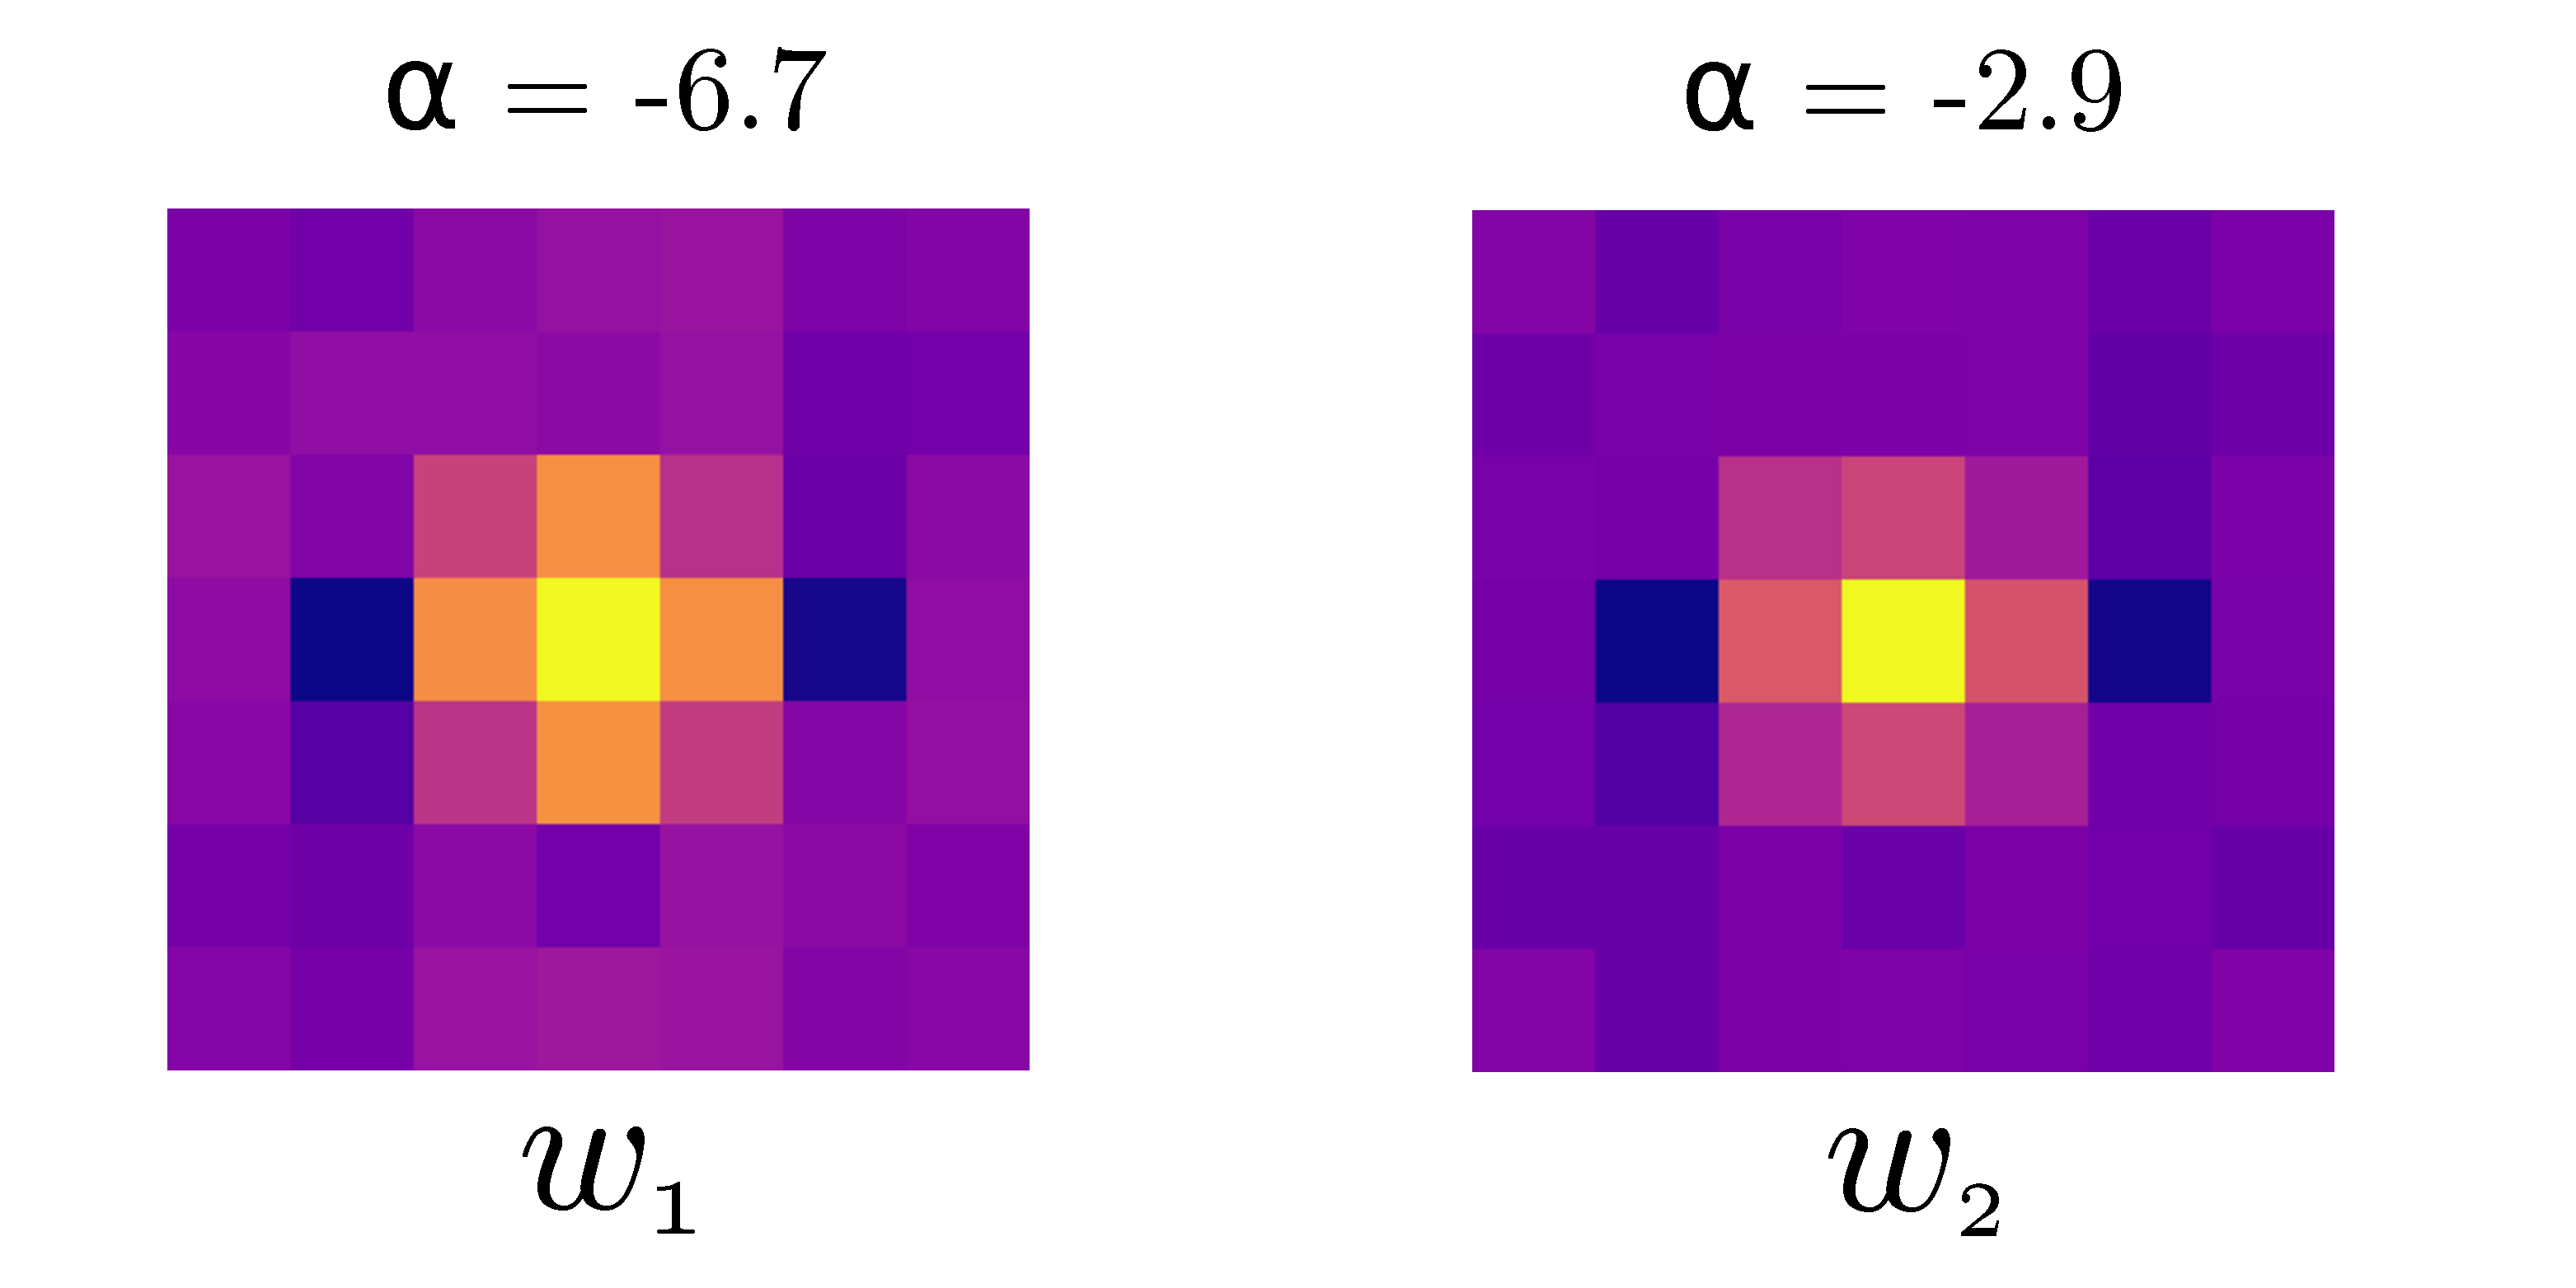
\includegraphics[width=0.36\linewidth]{parts/4-analyse_des_reseaux/deux_couches_pour_OPfondamentale/figures/square_fail.pdf}
    \vspace{1.0mm}
    \caption{ \centering État final du réseau $\mathcal{S}$MorphNetTanh à deux couches morphologiques, pour la fonction structurante cible carrée 3x3 et l'opération cible d'\textbf{érosion} sur la banque d'images d'entraînement MNIST, sans contrainte. Résultat : échec.}
    \label{fig:square_fail}
  \end{center}
\end{figure}

\vspace{-0.4mm}
On remarque que, pour cet exemple, le réseau a mal convergé, car la forme des noyaux est peu reconnaissable, les paramètres de contrôle $\alpha$ sont de très faible amplitude, et on obtient une valeur de perte sur les prédictions élevée, de l'ordre de $10^{-3}$. \\

\vspace{-1.0mm}
\noindent On peut cependant, pour cette structure carrée 3x3, tenter de la forcer à mieux converger, en lui imposant une contrainte dans la fonction de perte \textit{loss}. Dans notre cas, on prendra la contrainte sur la norme $L_1$, avec $l_c = 0$ (formule \ref{erreur_norm}). La convergence devient alors bien meilleure : on obtient l'état final des deux couches suivant, illustré fig. \ref{fig:square_success}.


\newpage

%figure
\begin{figure}[!htp]
  \begin{center}
    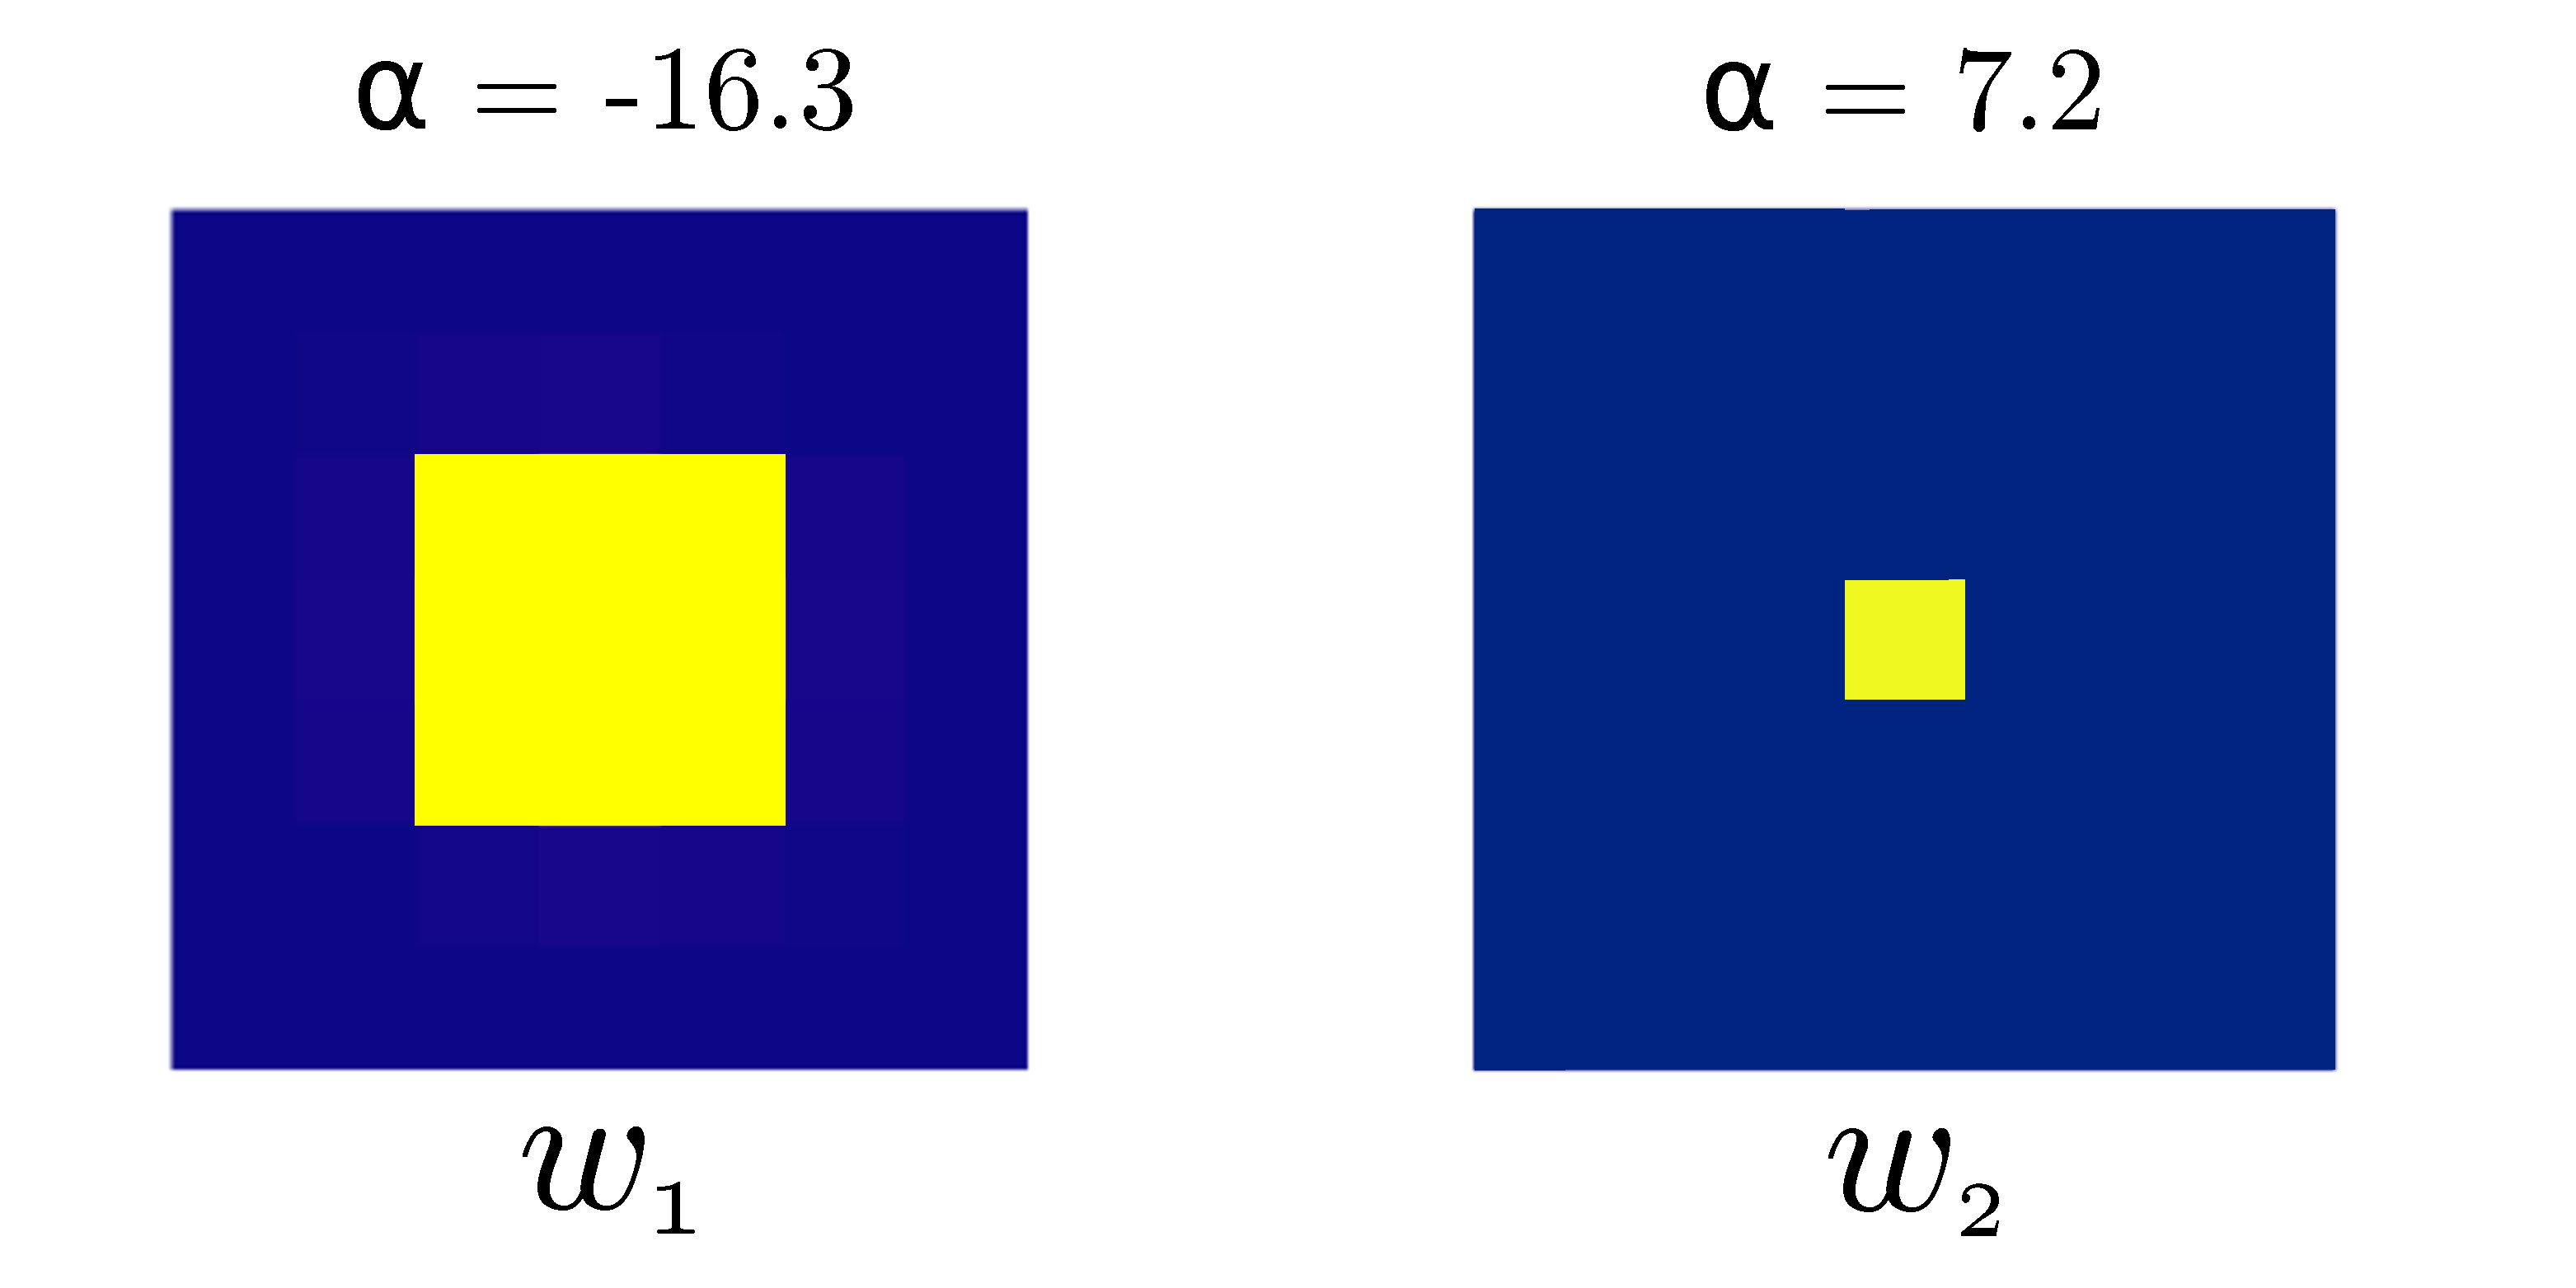
\includegraphics[width=0.36\linewidth]{parts/4-analyse_des_reseaux/deux_couches_pour_OPfondamentale/figures/square_success.pdf}
    \vspace{1.0mm}
    \caption{ \centering État final du réseau $\mathcal{S}$MorphNetTanh à deux couches morphologiques, pour la fonction structurante cible carrée 3x3 et l'opération cible d'\textbf{érosion} sur la banque MNIST, avec une contrainte des noyaux sur la norme $L_1$. Résultat : succès.}
    \label{fig:square_success}
  \end{center}
\end{figure}

\vspace{-0.2mm}
On remarque que, pour cet exemple encore, le réseau a, cette fois-ci, bien convergé, grâce à l'ajout de cette contrainte des noyaux $w$ sur la norme $l_1$ : la forme des noyaux est très reconnaissable (le premier noyau a la forme de la structure cible i.e. le carré 3x3, et le second a la forme de l'identité i.e. un unique pixel distinguable au centre du support), les paramètres de contrôle $\alpha$ ont une plus grande amplitude, et on obtient une valeur de perte sur les prédictions du réseau bien plus faible, de l'ordre de $10^{-6}$. \\

%\vspace{-0.0mm}
\noindent Parmi les deux groupes << succès >> et << échecs >> des résultats de convergence que l'on a distingués sur l'ensemble des expériences, en examinant uniquement les \textit{succès}, on peut remarquer que l'amplitude des paramètres $\alpha$ n'est jamais très élevée (de l'ordre de 10), et aussi, mais surtout, que l'on obtient \textit{toujours} la configuration des couches suivantes : la première couche a un noyau $w_1$ de la forme de la fonction structurante cible, avec un $\alpha$ associé négatif, et la seconde couche a un noyau $w_2$ de la forme de l'identité (un seul pixel actif), avec un $\alpha$ associé positif. On n'obtient jamais de composition originale ou plus complexe sur ces succès, même avec l'aide de contraintes pour favoriser certaines configurations, et on a toujours le même ordre : d'abord la structure cible, puis l'identité. C'est le cas par exemple du carré 3x3, aidé de la contrainte $L_1$, telle qu'illustrée figure \ref{fig:square_success} (d'abord carré 3x3, puis identité).

\vspace{3.6mm}
